% v2-acmlarge-sample.tex, dated March 6 2012
% This is a sample file for ACM large trim journals
%
% Compilation using 'acmlarge.cls' - version 1.3, Aptara Inc.
% (c) 2011 Association for Computing Machinery (ACM)
%
% Questions/Suggestions/Feedback should be addressed to => "acmtexsupport@aptaracorp.com".
% Users can also go through the FAQs available on the journal's submission webpage.
%
% Steps to compile: latex, bibtex, latex latex
%
\documentclass[prodmode,acmtap]{acmlarge}

% Metadata Information
\acmVolume{2}
\acmNumber{3}
\acmArticle{1}
\articleSeq{1}
\acmYear{2010}
\acmMonth{5}

% Package to generate and customize Algorithm as per ACM style
\usepackage[ruled]{algorithm2e}
\usepackage[spanish]{babel}
\usepackage[utf8]{inputenc}
\SetAlFnt{\algofont}
\SetAlCapFnt{\algofont}
\SetAlCapNameFnt{\algofont}
\SetAlCapHSkip{0pt}
\IncMargin{-\parindent}
\renewcommand{\algorithmcfname}{ALGORITHM}

% Page heads
\markboth{D. Pineo, C. Ware and S. Fogarty}{Resumen:  PseudoRandom Bit Generator Based on Couple Chaotic Systems and its Applications in Stream Cipher Cryptography}

% Title portion
\title{Resumen:  Chaos Applications in Telecomunications}
\author{Marcos Daniel Calderón Calderón \affil{CIMAT}
}
% NOTE! Affiliations placed here should be for the institution where the
%       BULK of the research was done. If the author has gone to a new
%       institution, before publication, the (above) affiliation should NOT be changed.
%       The authors 'current' address may be given in the "Author's addresses:" block (below).
%       So for example, Mr. Fogarty, the bulk of the research was done at UIUC, and he is
%       currently affiliated with NASA.

\begin{abstract}
Resumen de Libro.
\end{abstract}



\begin{document}




\maketitle

\section{El camino hacia los fractales.}

\subsection{El principio de Feedback.}


Es un error hablar de Fractales sin tener en cuenta los procesos dinámicos que los generan. 
Los procesos con Feedback son fundamentales en las ciencias exactas. Estos fueron introducido por IsaacNewton y por Gottfried Leibniz hace aproximadamente 300 años en forma de leyes dinámicas.  Dichas leyes determinan la localización y la velocidad de una particula en un instante de tiempo. El movimiento de la partículoa es entonces entendido como el desarrollo de una ley dinámica. 

Una máquina de Feedback se puede representar por el siguiente esquema.

\begin{figure}[H]
\centering
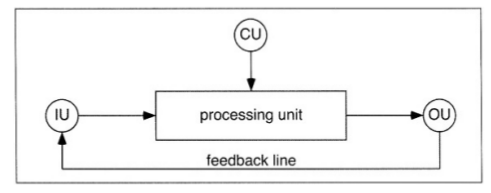
\includegraphics[width=7cm]{fe.png}
\caption{Máquina de Feedback.}
\label{fo}
\end{figure}


Un ejemplo sencillo de una máquina Feedback es un experimento donde una cámara de video está grabando la pantalla de una televisión, además, la señal que capta la cámara se muestra al mismo tiempo en la televisión, de esta manera, por el proceso de retroalimentación, en la televisión se observa un patrón que consiste en un monitor adentro de un monitor: cada uno de los monitores es reproducido adentro de otro monitor y cada uno es más pequeño que el anterior.
Cuando la distancia de la cámara es menor y no se ve el monitor, lo que ocurre es un efecto de zoom de los objetos captados. El efecto de el proceso puede ser descrito como un proceo dinámico de compresión. 




\end{document}
% End of v2-acmlarge-sample.tex (March 2012) - Gerry Murray, ACM
